\documentclass[preview]{standalone}
\usepackage{tikz}
\usetikzlibrary{decorations.pathreplacing}

\begin{document}
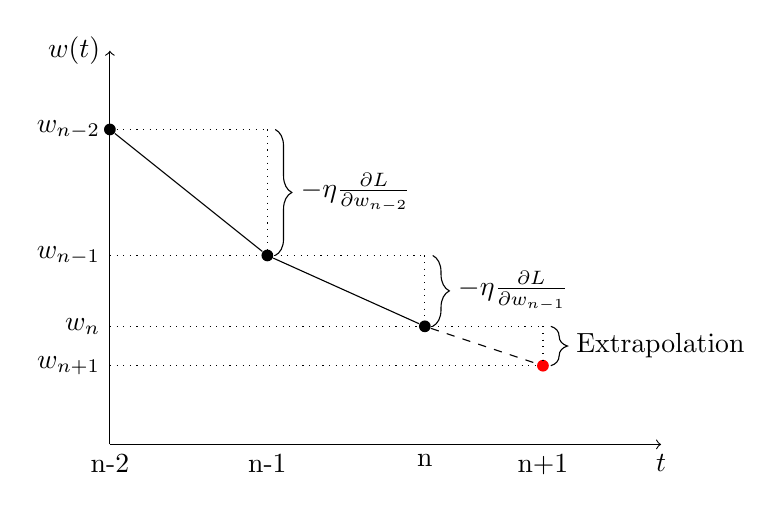
\begin{tikzpicture}
% horizontal axis
\draw[->] (0,0) -- (7,0) node[anchor=north] {$t$};
% vertical axis
\draw[->] (0,0) -- (0,5) node[anchor=east] {$w(t)$};
% points
\node (p1) at (0,4.0) [circle, fill, inner sep=1.5pt]{}; 
\node (p2) at (2,2.4) [circle, fill, inner sep=1.5pt]{}; 
\node (p3) at (4,1.5) [circle, fill, inner sep=1.5pt]{}; 
\node (p4) at (5.5,1.0) [circle, fill, inner sep=1.5pt,red]{}; 
% x-labels
\node (n1) at (0,0) [anchor=north] {n-2};
\node (n2) at (2,0) [anchor=north] {n-1};
\node (n3) at (4,0) [anchor=north] {n};
\node (n4) at (5.5,0) [anchor=north] {n+1};
% y-labels
\draw (0,1.0) node[anchor=east] {$w_{n+1}$};
\draw (0,1.5) node[anchor=east] {$w_{n}$};
\draw (0,2.4) node[anchor=east] {$w_{n-1}$};
\draw (0,4.0) node[anchor=east] {$w_{n-2}$};
% lines
\draw[] (p1) -- (p2);
\draw[] (p2) -- (p3);
\draw[dashed] (p3) -- (p4);
% y-braces
\draw [decorate,decoration={brace,amplitude=6pt,mirror},xshift=0.1cm,yshift=0cm] (2.0,2.4) -- (2.0,4.0) node [anchor=west,midway,xshift=0.2cm,yshift=0cm] {$-\eta\frac{\partial L}{\partial w_{n-2}}$};
\draw [decorate,decoration={brace,amplitude=6pt,mirror},xshift=0.1cm,yshift=0cm] (4.0,1.5) -- (4.0,2.4) node [anchor=west,midway,xshift=0.2cm,yshift=0cm] {$-\eta\frac{\partial L}{\partial w_{n-1}}$};
\draw [decorate,decoration={brace,amplitude=6pt,mirror},xshift=0.1cm,yshift=0cm] (5.5,1.0) -- (5.5,1.5) node [anchor=west,midway,xshift=0.2cm,yshift=0cm] {Extrapolation};
% dotted lines
\draw[dotted] (0.0,4.0) -- (2.0,4.0);
\draw[dotted] (2.0,2.4) -- (4.0,2.4);
\draw[dotted] (2.0,4.0) -- (2.0,2.4);
\draw[dotted] (4.0,2.4) -- (4.0,1.5);
\draw[dotted] (4.0,1.5) -- (5.5,1.5);
\draw[dotted] (5.5,1.5) -- (5.5,1.0);
\draw[dotted] (0,1.0) -- (p4);
\draw[dotted] (0,1.5) -- (p3);
\draw[dotted] (0,2.4) -- (p2);
\end{tikzpicture}
\end{document}
